%% LyX 2.0.6 created this file.  For more info, see http://www.lyx.org/.
%% Do not edit unless you really know what you are doing.
\documentclass[english]{article}
\usepackage[T1]{fontenc}
\usepackage[latin9]{inputenc}
\usepackage{geometry}
\geometry{verbose,tmargin=2cm,bmargin=3cm,lmargin=1.5cm,rmargin=1.5cm}
\usepackage{array}
\usepackage{multirow}
\usepackage{enumerate}
\usepackage{amsmath}
\usepackage{amsfonts}
\usepackage{amssymb}
\usepackage{verbatim}
\usepackage{appendix}
\usepackage{mathtools}
\usepackage{caption}
\newcommand*\diff{\mathop{}\!\mathrm{d}}
\renewcommand{\vec}[1]{\boldsymbol{\mathbf{#1}}} % Vectors
\newcommand{\mat}[1]{\boldsymbol{\mathbf{#1}}} % Matrices
\PassOptionsToPackage{normalem}{ulem}
\usepackage{ulem}
\usepackage{mathrsfs}

\usepackage{algorithm}
\usepackage[noend]{algpseudocode}
\usepackage{tikz-qtree}

\makeatletter
\def\BState{\State\hskip-\ALG@thistlm}
\makeatother

%%%%%%%%%%%%%%%%%%%%%%%%%%%%%% LyX specific LaTeX commands.
%% Because html converters don't know tabularnewline
\providecommand{\tabularnewline}{\\}

%%%%%%%%%%%%%%%%%%%%%%%%%%%%%% User specified LaTeX commands.
\usepackage{tikz}
\usepackage{babel}
\renewcommand{\labelitemi}{$\diamond$}
\newcommand\T{\rule{0pt}{2.6ex}}       % Top strut
\newcommand\B{\rule[-1.2ex]{0pt}{0pt}} % Bottom strut


\makeatother

\begin{document}

\title{COMP8620: MC-AIXI-CTW\\Group 3}
\author{Jarryd Martin, John Aslanides, Yadunandan Sannappa, Nrupendra Rao, Cheng Yu, Ryk Budzynski}
\date{October 2015}

\maketitle

\section{Introduction}

\subsection{Domains}
The domains assigned to group 3 are as follows:
$$\text{Pacman, Tic-Tac-Toe, Biased Rock-Paper-Scissor, Extended Tiger, Cheesemaze}$$

\subsection{Files}
The report archive should contian the following:
\begin{verbatim}
MC-AIXI-CTW-Grp3.zip
    \report
        report.pdf // this report
        report.tex
        cheesemaze_01.png // results plots
        extended_tiger_01.png
        biased_rock_paper_scissor_01.png
        tic_tac_toe_01.png
        pacman_01.png
    \src
        main.hpp
        main.cpp
        environment.hpp
        environment.cpp
        agent.hpp
        agent.cpp
        search.hpp
        search.cpp
        predict.hpp
        predict.cpp
        util.hpp
        util.cpp
        README.md
        cheesemaze.conf // environment configuration files
        rockpaper.conf
        tictactoe.conf
        coinflip.conf
        tiger.conf

        
\end{verbatim}

\subsection{User Manual}

\section{MC-AIXI-CTW Implementation}

\subsection{Environments}
\subsubsection{Cheesemaze}
\subsubsection{Extended Tiger}
\subsubsection{Biased Rock-Paper-Scissor}
\subsubsection{Tic-Tac-Toe}
\subsubsection{Pacman}

\subsection{Monte Carlo Tree Search (MCTS) Algorithm}

\begin{enumerate}[a)]
\item Source code files
\item Class structure (SearchNode, DecisionNode, ChanceNode, ...)
\item Description of the algorithm (Veness...)
\end{enumerate}

\subsection{Context Tree Weighting (CTW)}

\section{Simulation Results}
\subsection{Cheesemaze}
\begin{itemize}
\item Experimental setup ... \\
Any simulation provided should include detailed description of experimental setup; selected parameters of algorithms and examples; and concise interpretations of obtained simulation results. \\

\begin{tabular}{|l|l|l|c}
\hline
Environment & MCTS & CTW \\
\hline
1 & $m = 100$      & $\text{ct-depth} = 96$ \\
\hline
  & $C = \sqrt{2}$ &  \\
\hline
\end{tabular}

\item Plots ... \\
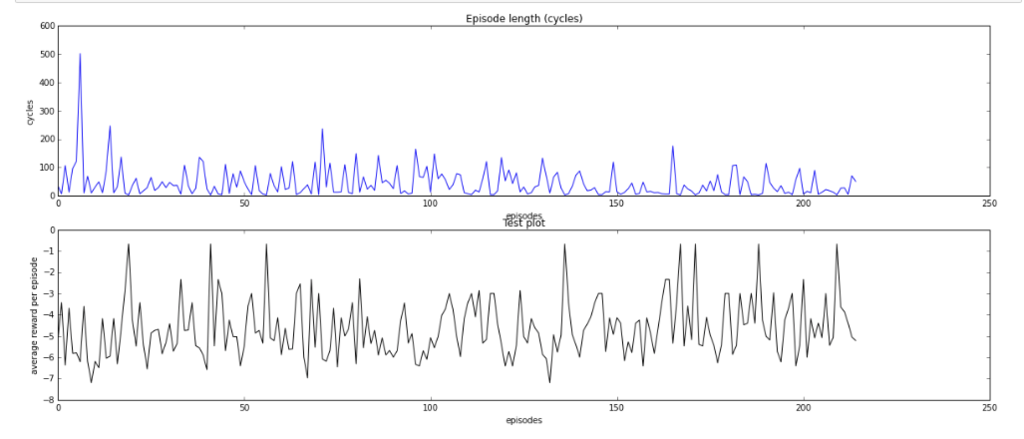
\includegraphics[scale=0.4]{./cheesemaze_01}
\item Interpretation of Results
\end{itemize}

\subsection{Extended Tiger}
Experimental setup ... \\
Plots ...
\subsection{Biased Rock-Paper-Scissor}
Experimental setup ... \\
Plots ...
\subsection{Tic-Tac-Toe}
Experimental setup ... \\
Plots ...
\subsection{Pacman}
Experimental setup ... \\
Plots ...
\section{Cross Domain Simulation Results}
Cheesemaze and Extended Tiger

\section{Possible Other things}
Cross domain simulation on more difficult environments... \\
Separate CTW for Obs and Rews...

\end{document}
